% =============================================================================
%  EE4311 [2610] Project 1 -- Sugeno Fuzzy PD Controller (5x5)
%  Baseline report template.  Team 16.
%
%  Compile:  pdflatex p1_team16 && bibtex p1_team16 && pdflatex p1_team16 (x2)
%  or:       latexmk -pdf p1_team16
%
%  RULES (from worksheet Section 7.3):
%    - NO student names anywhere in the report. Matric numbers only.
%    - Front matter order: cover page, contents, list of individual contributions.
%    - Back matter order:  declarations, references, appendices.
%    - Main body between front matter and back matter, roughly 10-30 pages.
%    - Output file name must be p1_team16.pdf (lowercase).
% =============================================================================
\documentclass[11pt,a4paper]{article}

% ---------------------------------------------------------------- packages ---
\usepackage[T1]{fontenc}
\usepackage[utf8]{inputenc}
\usepackage[margin=2.5cm]{geometry}
\usepackage{graphicx}
\usepackage{booktabs}
\usepackage{array}
\usepackage{amsmath,amssymb}
\usepackage{siunitx}
\usepackage[font=small,labelfont=bf]{caption}
\usepackage{subcaption}
\usepackage{xcolor}
\usepackage{enumitem}
\usepackage{float}
\usepackage[hidelinks]{hyperref}
\hypersetup{pageanchor=false} % titlepage and page 1 would otherwise clash
\usepackage{fancyhdr}
\usepackage{titlesec}
\usepackage{pgfplots}
\pgfplotsset{compat=1.17}

% ------------------------------------------------------------------ macros ---
\newcommand{\todo}[1]{\textcolor{red}{\textbf{[TODO: #1]}}}
\newcommand{\degC}{\ensuremath{^\circ}}
\newcommand{\gam}{\ensuremath{\gamma}}
\newcommand{\gamdot}{\ensuremath{\dot{\gamma}}}
\newcommand{\ts}{\ensuremath{t_s}}
\newcommand{\overshoot}{\ensuremath{M_p}}
\newcommand{\sse}{\ensuremath{e_{ss}}}

\graphicspath{{figures/}}

\setlength{\headheight}{14pt}
\pagestyle{fancy}
\fancyhf{}
\rhead{EE4311 Project 1 -- Team 16}
\lhead{\leftmark}
\cfoot{\thepage}

\titleformat{\section}{\normalfont\large\bfseries}{\thesection}{0.8em}{}
\titleformat{\subsection}{\normalfont\normalsize\bfseries}{\thesubsection}{0.8em}{}

% =============================================================================
\begin{document}

% =============================================================================
% FRONT MATTER
% =============================================================================
\begin{titlepage}
\centering
\vspace*{2cm}

{\scshape\large EE4311 [2610] -- Intelligent Control Systems\par}
\vspace{0.5cm}
{\scshape\large Project 1\par}

\vspace{2cm}
\rule{\textwidth}{1pt}
\vspace{0.5cm}
{\huge\bfseries Sugeno Fuzzy PD Controller (5$\times$5) for an\\[0.3em]
Inverted Pendulum on a Slope\par}
\vspace{0.5cm}
\rule{\textwidth}{1pt}

\vspace{3cm}
{\large Team 16\par}
\vspace{0.5cm}

% --- Matric numbers only. Do NOT put names here. ---
\begin{tabular}{c}
\toprule
Matriculation Number \\
\midrule
\todo{matric no. of member 1} \\
\todo{matric no. of member 2} \\
\bottomrule
\end{tabular}

\vfill
{\large \todo{submission date}\par}
\end{titlepage}

\clearpage
\tableofcontents
\clearpage

% ------------------------------------------------- individual contributions ---
\section*{List of Individual Contributions}
\addcontentsline{toc}{section}{List of Individual Contributions}

% Significant contributions only: experimentation, analysis, and reporting of
% results. Writing/formatting and preliminary coding are NOT significant.
\begin{table}[H]
\centering
\small
\begin{tabular}{@{}p{2.6cm}p{3.4cm}p{9.2cm}@{}}
\toprule
\textbf{Matric no.} & \textbf{Area} & \textbf{Contribution (point form)} \\
\midrule
\todo{matric 1} & Tuning method A & \todo{one line per contribution: e.g. designed and ran the 11 experiments on input scaling; produced the data in Appendix~\ref{app:data}} \\
                &                 & \todo{contribution 2} \\[0.4em]
\todo{matric 2} & Tuning method B & \todo{contribution 1} \\
                &                 & \todo{contribution 2} \\
\bottomrule
\end{tabular}
\caption{Individual contributions. Each member must have at least two
investigated tuning methods (worksheet Section 8, item 2).}
\label{tab:contributions}
\end{table}

\clearpage
% =============================================================================
% MAIN BODY
% =============================================================================

\section{Introduction}
\label{sec:intro}

This report investigates a Sugeno (Takagi--Sugeno) \cite{takagi1985fuzzy}
fuzzy PD controller that
balances an inverted pendulum mounted on a cart on a \SI{30}{\degree} slope.
The plant is the same as in Lab~2 but with different cart mass, pendulum mass
and pendulum length, and the controller is implemented as a 5$\times$5 rule
base with crisp consequents instead of a Mamdani inference system.

The control objective is stated directly in terms of closed-loop response
characteristics:
\begin{enumerate}[label=(\arabic*),leftmargin=*]
  \item settling time $\ts \le \SI{1}{\s}$ for every initial angle
        $\gam_0 \in \{-10\degC, -5\degC, 5\degC, 10\degC\}$;
  \item negligible overshoot $\overshoot$ in $\gam$;
  \item steady-state angle as close to zero as possible;
  \item negligible oscillation in all responses.
\end{enumerate}
Cart displacement and cart velocity are explicitly outside the scope of the
assessment.

\paragraph{Contributions of this report.}
\todo{3--4 sentences: what tuning methods are studied, what the best model
achieves in \si{\s} and \si{\degree}, and what the main insight is. Written
last, once the numbers exist.}

\paragraph{Organisation.}
Section~\ref{sec:defs} defines the plant parameters and the fuzzy inference
system. Section~\ref{sec:controller} derives the PD error signals.
Section~\ref{sec:method} defines the simulation setup and the performance
metrics used throughout. Section~\ref{sec:baseline} reports the baseline model
from Lab~2. Section~\ref{sec:tuning} presents the tuning investigations and
their analysis, Section~\ref{sec:best} the combined best model, and
Section~\ref{sec:conclusion} concludes.

\section{System Definition and Fuzzy Inference System}
\label{sec:defs}

\subsection{Random seed and plant parameters}
\label{sec:params}

The random seed is fixed to the sum of the numeric digits of the team's
matriculation numbers, $\mathrm{rng}(\mathrm{sum}([286716, 284748]))$, so that
the plant parameters below are reproducible:
\begin{verbatim}
constants.G      = 9.8;                      % gravity, m/s^2
constants.M_CART = rand()*1   + 0.5;         % cart mass, kg
constants.M_PEND = rand()*0.2 + 1.4;         % pendulum mass, kg
constants.L_PEND = rand()*0.2 + 0.9;         % pendulum length, m
constants.PHI    = 30;                       % slope angle, deg
\end{verbatim}

\begin{table}[H]
\centering
\small
\begin{tabular}{@{}llll@{}}
\toprule
\textbf{Symbol} & \textbf{Quantity} & \textbf{Value} & \textbf{Unit} \\
\midrule
$g$            & gravitational acceleration & 9.8 & \si{\m\per\s\squared} \\
$\phi$         & slope angle                & 30  & \si{\degree} \\
$m_c$          & cart mass                  & \todo{value} & \si{\kg} \\
$m_p$          & pendulum mass              & \todo{value} & \si{\kg} \\
$L$            & pendulum length            & \todo{value} & \si{\m} \\
$W$            & weight component along slope & \todo{value} & \si{\N} \\
$e$            & proportional error universe & $[-20, 20]$ & \si{\degree} \\
$\dot e$       & derivative error universe   & $[-80, 80]$ & \si{\degree\per\s} \\
$f$            & output force universe       & $[-50, 50]$ & \si{\N} \\
\bottomrule
\end{tabular}
\caption{Plant and controller constants. Values obtained from the fixed seed.}
\label{tab:constants}
\end{table}

The weight force acting down the slope is the disturbance the controller must
compensate for at steady state,
\begin{equation}
  W = g \sin\phi \, (m_c + m_p),
  \label{eq:weight}
\end{equation}
which is used as a tuning reference: the fuzzy output at zero error must be
able to generate a force of at least this magnitude, otherwise the pendulum
cannot be held off-centre on the slope.

\subsection{Membership functions}
\label{sec:mfs}

Both inputs use five trapezoidal membership functions (NB, NS, ZO, PS, PB)
parameterised by $(a,b,c,d)$; the output uses five Sugeno \emph{constant}
membership functions, added with \texttt{addMF}~\cite{mathworks_sugfis}. Table~\ref{tab:mfs} lists the baseline parameters, which
are carried over from Lab~2, with the two additional terms per input
distributed evenly around the Lab~2 nodes ($\pm 2.6\degC$ for the proportional
error and $\pm 35\,\si{\degree\per\s}$ for the derivative error). The crisp output
values are distributed evenly over the universe.

\begin{table}[H]
\centering
\small
\begin{tabular}{@{}llll@{}}
\toprule
\textbf{Term} & \textbf{Proportional error $[a,b,c,d]$ (\si{\degree})}
              & \textbf{Derivative error $[a,b,c,d]$ (\si{\degree\per\s})}
              & \textbf{Force $f$ (\si{\N})} \\
\midrule
NB & $[-20,-20,-10,-2.6]$ & $[-80,-80,-60,-35]$ & $-50$ \\
NS & $[-10,-2.6,-2.6,0]$  & $[-60,-35,-35,0]$   & $-25$ \\
ZO & $[-2.6,0,0,2.6]$     & $[-35,0,0,35]$      & $0$   \\
PS & $[0,2.6,2.6,10]$     & $[0,35,35,60]$      & $25$  \\
PB & $[2.6,10,20,20]$     & $[35,60,80,80]$     & $50$  \\
\bottomrule
\end{tabular}
\caption{Baseline membership function parameters (Sugeno, 5$\times$5).}
\label{tab:mfs}
\end{table}

\begin{figure}[H]
\centering
\includegraphics[width=\textwidth]{p1_parameters.pdf}
\caption{Baseline membership functions for the proportional error, derivative
error and crisp output force, together with the resulting control surface.}
\label{fig:params}
\end{figure}

\subsection{Rule base}
\label{sec:rules}

The rule base is a 5$\times$5 PD-style table with a monotone diagonal: the
output magnitude increases with the magnitude of both the proportional error
and the derivative error. Table~\ref{tab:rules} tabulates the consequents;
each cell is one rule of the form
\texttt{p==X \& d==Y => f==Z}.

\begin{table}[H]
\centering
\small
\begin{tabular}{@{}c ccccc@{}}
\toprule
 & \multicolumn{5}{c}{\textbf{derivative error} $d$} \\
\cmidrule(lr){2-6}
\textbf{proportional error} $p$ & NB & NS & ZO & PS & PB \\
\midrule
NB & NB & NB & NB & NS & ZO \\
NS & NB & NB & NS & ZO & PS \\
ZO & NB & NS & ZO & PS & PB \\
PS & NS & ZO & PS & PB & PB \\
PB & ZO & PS & PB & PB & PB \\
\bottomrule
\end{tabular}
\caption{Rule base (output force term for each antecedent pair).}
\label{tab:rules}
\end{table}

\subsection{Inference methods}
\label{sec:methods}

The Sugeno system uses the operator set from the lecture
(Table~\ref{tab:inference})~\cite{passino1998fuzzy,ross2010fuzzy}. Because the consequents are crisp constants, the
aggregated output is a weighted average of the firing strengths, which makes
the defuzzified force a cheap and smooth function of $(p,d)$.

\begin{table}[H]
\centering
\small
\begin{tabular}{@{}lll@{}}
\toprule
\textbf{Stage} & \textbf{Method} & \textbf{Interpretation} \\
\midrule
And            & \texttt{min}      & antecedent conjunction \\
Or             & \texttt{max}      & antecedent disjunction \\
Implication    & \texttt{prod}     & Sugeno only supports \texttt{prod} \\
Aggregation    & \texttt{sum}      & combine rule consequents \\
Defuzzification& \texttt{wtaver}   & weighted average of crisp consequents \\
\bottomrule
\end{tabular}
\caption{Fuzzy inference settings.}
\label{tab:inference}
\end{table}

\section{Controller}
\label{sec:controller}

The controller is a fuzzy PD law~\cite{astrom2006feedback} with the desired state $(\gam^\ast, \gamdot^\ast) = (0,0)$:
\begin{align}
  p &= \gam^\ast - \gam = -\gam, & d &= \gamdot^\ast - \gamdot = -\gamdot, \\
  f &= \mathrm{evalfis}(\mathrm{fis}, [p, d]), & f &\leftarrow \mathrm{clip}(f, -50, 50).
\end{align}
The output is saturated at $\pm\SI{50}{\N}$ to mimic the actuator limit of the
real system. The proportional error supplies the restoring effort and the
derivative error provides damping; because both inputs are fed through the same
rule table, the effective closed-loop behaviour is that of a non-linear PD
controller whose gains vary over the operating region.

\paragraph{Expected behaviour.}
\todo{argue qualitatively what the surface in Figure~\ref{fig:params} implies:
where the gain is large, where the dead-zone-like ZO region is, and why a
uniform output distribution should give a symmetric response. This paragraph
motivates the tuning hypotheses in Section~\ref{sec:tuning}.}

\section{Method: Simulation and Performance Metrics}
\label{sec:method}

\subsection{Simulation setup}
\label{sec:sim}

The plant is integrated with a fixed-step forward Euler scheme from the
Euler--Lagrange equations of the pendulum--cart on the slope. Table~\ref{tab:sim}
lists the settings; note that the controller runs every 5 simulation steps
(\SI{50}{\ms} control period), so the plant is driven by a zero-order hold.
Friction is included on both the cart and the pendulum joint.

\begin{table}[H]
\centering
\small
\begin{tabular}{@{}lll@{}}
\toprule
\textbf{Parameter} & \textbf{Value} & \textbf{Meaning} \\
\midrule
$\Delta t$          & \SI{0.01}{\s}  & integration / simulation step \\
$T_{\text{total}}$  & \SI{5}{\s}     & simulated horizon \\
controller period   & $5\Delta t = \SI{50}{\ms}$ & zero-order hold \\
$k_{f,\text{cart}}$ & 3              & cart friction coefficient \\
$k_{f,\text{pend}}$ & $1\times10^{-4}$ & pendulum friction coefficient \\
$\gam_0$            & $\{-10,-5,5,10\}\degC$ & initial angles \\
\bottomrule
\end{tabular}
\caption{Simulation settings.}
\label{tab:sim}
\end{table}

\subsection{Performance metrics}
\label{sec:metrics}

All comparisons in this report use the same four metrics, each computed from
the simulated $\gam(t)$ and $f(t)$:
\begin{description}[leftmargin=*,style=nextline]
  \item[Settling time $\ts$] the first time after which $|\gam|$ stays within
        the $\pm\SI{1}{\degree}$ band for the remainder of the response.
  \item[Overshoot $\overshoot$] the maximum excursion of $\gam$ beyond zero in
        the direction opposite to $\gam_0$, normalised by $|\gam_0|$.
  \item[Steady-state error $\sse$] mean of $|\gam(t)|$ over the last
        \SI{1}{\s} of the simulation.
  \item[Oscillation] peak-to-peak amplitude of $\gam$ after $\ts$, or
        equivalently the number of zero crossings of $\gam$ in the last
        \SI{2}{\s}.
\end{description}

\paragraph{Reproducibility.}
\todo{state that every number in this report is produced by the submitted
worksheet with the fixed seed, and name the script that generates the sweep
tables (Appendix~\ref{app:code}).}

\section{Baseline Results}
\label{sec:baseline}

\subsection{Figures of merit}
\label{sec:baseline-metrics}

\begin{table}[H]
\centering
\small
\begin{tabular}{@{}cccccc@{}}
\toprule
$\gam_0$ (\si{\degree}) & $\ts$ (\si{\s}) & $\overshoot$ (\si{\%}) & $\sse$ (\si{\degree}) & Oscillation & Verdict \\
\midrule
$-10$ & \todo{} & \todo{} & \todo{} & \todo{} & \todo{} \\
$-5$  & \todo{} & \todo{} & \todo{} & \todo{} & \todo{} \\
$5$   & \todo{} & \todo{} & \todo{} & \todo{} & \todo{} \\
$10$  & \todo{} & \todo{} & \todo{} & \todo{} & \todo{} \\
\bottomrule
\end{tabular}
\caption{Baseline performance against the requirements ($\ts \le \SI{1}{\s}$,
negligible overshoot, $\sse \to 0$).}
\label{tab:baseline}
\end{table}

\begin{figure}[H]
\centering
\includegraphics[width=\textwidth]{p1_responses.pdf}
\caption{Baseline responses for the four initial angles: angle $\gam$, angular
velocity $\gamdot$ and cart force $f$. Dashed vertical lines mark $\ts$.}
\label{fig:baseline}
\end{figure}

\subsection{Interpretation}
\label{sec:baseline-interpretation}

\todo{Diagnose the baseline from Table~\ref{tab:baseline} and
Figure~\ref{fig:baseline}: which requirement fails, on which initial angle, and
what in the membership functions plausibly causes it (e.g.\ the ZO
dead-zone width sets the steady-state error, the NS/PS width sets the
oscillation, the output spacing sets the force resolution). Each claim here
becomes a testable hypothesis in Section~\ref{sec:tuning}.}

\section{Tuning Investigations}
\label{sec:tuning}

\paragraph{How to read this section.}
Each subsection states the tuning method, the hypothesis it tests, the
experimental design, the measured effect on the four metrics, and an
interpretation. Methods that do not help are reported as negative results,
because they constrain the search space and reveal which mechanism dominates.

\subsection{Method A: \todo{name of tuning method}}
\label{sec:method-a}

\paragraph{Motivation and hypothesis.} \todo{why this method was chosen, with
reference to the control surface or to the baseline diagnosis.}

\paragraph{Design.} \todo{which parameters were varied, over what range, how
many levels, everything else held constant, number of initial angles.}

\begin{table}[H]
\centering
\small
\begin{tabular}{@{}lcccccc@{}}
\toprule
\textbf{Setting} & \textbf{Parameter} & $\ts$ (\si{\s}) & $\overshoot$ (\si{\%}) & $\sse$ (\si{\degree}) & Oscillation & Note \\
\midrule
S1 & \todo{} & \todo{} & \todo{} & \todo{} & \todo{} & \todo{} \\
S2 & \todo{} & \todo{} & \todo{} & \todo{} & \todo{} & \todo{} \\
S3 & \todo{} & \todo{} & \todo{} & \todo{} & \todo{} & \todo{} \\
\bottomrule
\end{tabular}
\caption{Method A sweep. Metrics reported for the worst initial angle, or as
mean $\pm$ range over the four angles (state which).}
\label{tab:method-a}
\end{table}

\paragraph{Results and interpretation.} \todo{quantify the trend, explain the
mechanism, and state whether the hypothesis held.}

\subsection{Method B: \todo{name of tuning method}}
\label{sec:method-b}

\paragraph{Motivation and hypothesis.} \todo{}
\paragraph{Design.} \todo{}
\paragraph{Results and interpretation.} \todo{}

\subsection{Method C: Rule Weighting}
\label{sec:method-c}

\paragraph{Motivation and hypothesis.} The baseline diagnosis
(Section~\ref{sec:baseline-interpretation}) is that $\gam$ never settles: it
converges to a constant offset of roughly $1.8$--$1.9\degC$ for every initial
angle. The mechanism is structural, not a bad breakpoint choice: at the exact
origin $p{=}0,d{=}0$ only the single rule \texttt{p==ZO \& d==ZO => f==ZO}
fires (its neighbours evaluate to zero there, since \texttt{ZO} is a
triangular, not flat-topped, term), so the crisp output is forced to
$f{=}\SI{0}{\newton}$ whenever $\gam{=}0$. Since the slope contributes a
constant force \texttt{constants.WEIGHT} $\ne 0$ along the track, $0\,$N can
never be an equilibrium at $\gam{=}0$, and the baseline settles wherever the
blended output finally balances gravity instead -- away from the exact
origin, so the offset is unavoidable given the rule base's output levels.
Away from the origin, however, $2$--$4$ rules overlap (both inputs have
overlapping trapezoids), so the hypothesis tested here is: \emph{without
moving any membership-function breakpoint or crisp output level, can giving
each of the 25 rules its own weight $w_{ij}\in(0.02,1]$ bias which of the
overlapping rules dominates the \texttt{wtaver} blend enough to pull the true
equilibrium much closer to $\gam{=}0$, and speed up the approach to it?}

\paragraph{Design.} Each rule's trailing \texttt{addRule} weight argument was
parameterised as one entry of a $5\times5$ matrix \texttt{params.RULE\_W}
(rows/cols ordered NB,NS,ZO,PS,PB for $p,d$) and searched with MATLAB's
\texttt{fminsearch} (derivative-free Nelder--Mead, since the cost comes from
the non-smooth Euler--Lagrange simulation, not a closed form), started from
several random and warm-started restarts to avoid the many local minima of a
25-dimensional, non-convex search. The cost summed, over all four
$\gam_0$, an integral-squared-error term on $\gam(t)$ (weighted more heavily
after $t{=}\SI{0.5}{\s}$ and over the final \SI{1}{\s}, to push settling
speed and steady-state accuracy specifically), explicit penalties on
overshoot and final $\sse$, and a mild control-effort term. Three settings
were evaluated, because the first optimisation round produced a genuine
negative result that motivated a second (Section~\ref{sec:negative}
elaborates): \textbf{S1} baseline ($w_{ij}{=}1$ for all rules, i.e.\ no
weighting, equivalent to the original rule base since a uniform scale factor
cancels in \texttt{wtaver}); \textbf{S2} the above cost optimised with no
smoothness term; \textbf{S3} the same optimisation with two extra penalty
terms added, $\sum(\Delta f)^2$ (squared jump in cart force between
consecutive controller updates) and $\sum(\Delta\gamdot)^2$ restricted to the
second half of the run (residual angular-velocity oscillation), to explicitly
discourage chattering. All optimisations, and the reported metrics, use the
same fixed team seed and plant parameters as the rest of this report.

\begin{table}[H]
\centering
\small
\begin{tabular}{@{}lcccccc@{}}
\toprule
\textbf{Setting} & \textbf{Parameter} & $\ts$ (\si{\s}) & $\overshoot$ (\si{\%}) & $\sse$ (\si{\degree}) & Oscillation & Note \\
\midrule
S1 & baseline, $w_{ij}{=}1$ & $\infty$ & 21.6 (0--56.4) & 1.83 (1.76--1.94) & n/a (never settles) & steady bias, no chatter \\
S2 & optimised, tracking-only cost & 0.38 (0.14--0.70) & 3.8 (0--11.4) & 0.27 (0.23--0.34) & 1.08 (0.81--1.43) & severe $\gamdot$/force chatter \\
S3 (final) & optimised, + anti-chattering terms & 0.31 (0.24--0.40) & 8.7 (1.9--21.9) & 0.51 (0.44--0.60) & 1.11 (0.68--1.61) & smooth; adopted \\
\bottomrule
\end{tabular}
\caption{Method C settings. Metrics reported as mean (range) over the four
initial angles $\gam_0\in\{-10,-5,5,10\}\degC$. ``Oscillation'' is this
report's defined metric: peak-to-peak $\gam$ after $\ts$.}
\label{tab:method-c}
\end{table}

\paragraph{Results and interpretation.} The hypothesis held for settling
speed and steady-state error: rule weighting alone takes $\ts$ from $\infty$
to well under \SI{0.5}{\s} for every initial angle (S3), and cuts mean
$\sse$ by $72\%$ (from $1.83\degC$ to $0.51\degC$), by shifting the
equilibrium blend rather than any breakpoint. It does not reach zero
overshoot or zero $\sse$: because the single rule active at the exact origin
still always outputs $0\,$N regardless of its own weight, weighting can only
push the equilibrium \emph{close to} $\gam{=}0$, never exactly onto it, so a
small residual bias and a proportionally small overshoot on the way to it are
an expected floor for this method used alone (see
Section~\ref{sec:combination} for combining it with a crisp-value shift,
which \emph{can} move that zero-force point).

A second, more important finding is about the metric itself. Table
\ref{tab:method-c}'s own \emph{Oscillation} column (peak-to-peak $\gam$ after
$\ts$) is almost identical between S2 ($1.08\degC$ mean) and S3
($1.11\degC$ mean) -- it does not distinguish them at all, because $\gam$
looks essentially flat in both cases (Figure~\ref{fig:methodc} vs.\ the
equivalent S2 plot, not reproduced here for space). Yet S2's cart force was
visibly bang-banging between its saturation limits and its tail angular
velocity had standard deviation $3.70\degC/\text{s}$ (range
$3.55$--$3.81$), while S3's was $0.063\degC/\text{s}$ (range
$0.023$--$0.099$) -- a $\sim\!59\times$ reduction -- for a worse-looking
Oscillation number. This is a case where the worksheet's own advice (Section
8, item 3: \emph{``the metrics need to be reasonable and not placed for the
sake of measuring''}) is directly actionable: peak-to-peak $\gam$ misses
chattering that lives in $\gamdot$ and $f$, not $\gam$ itself, so two
purpose-built metrics -- $\max|\Delta f|$ between consecutive controller
updates and $\operatorname{std}(\gamdot)$ over the run's second half -- were
added specifically to catch it, and are what motivated rejecting S2 for S3
despite S2's better raw tracking numbers.

\begin{figure}[H]
\centering
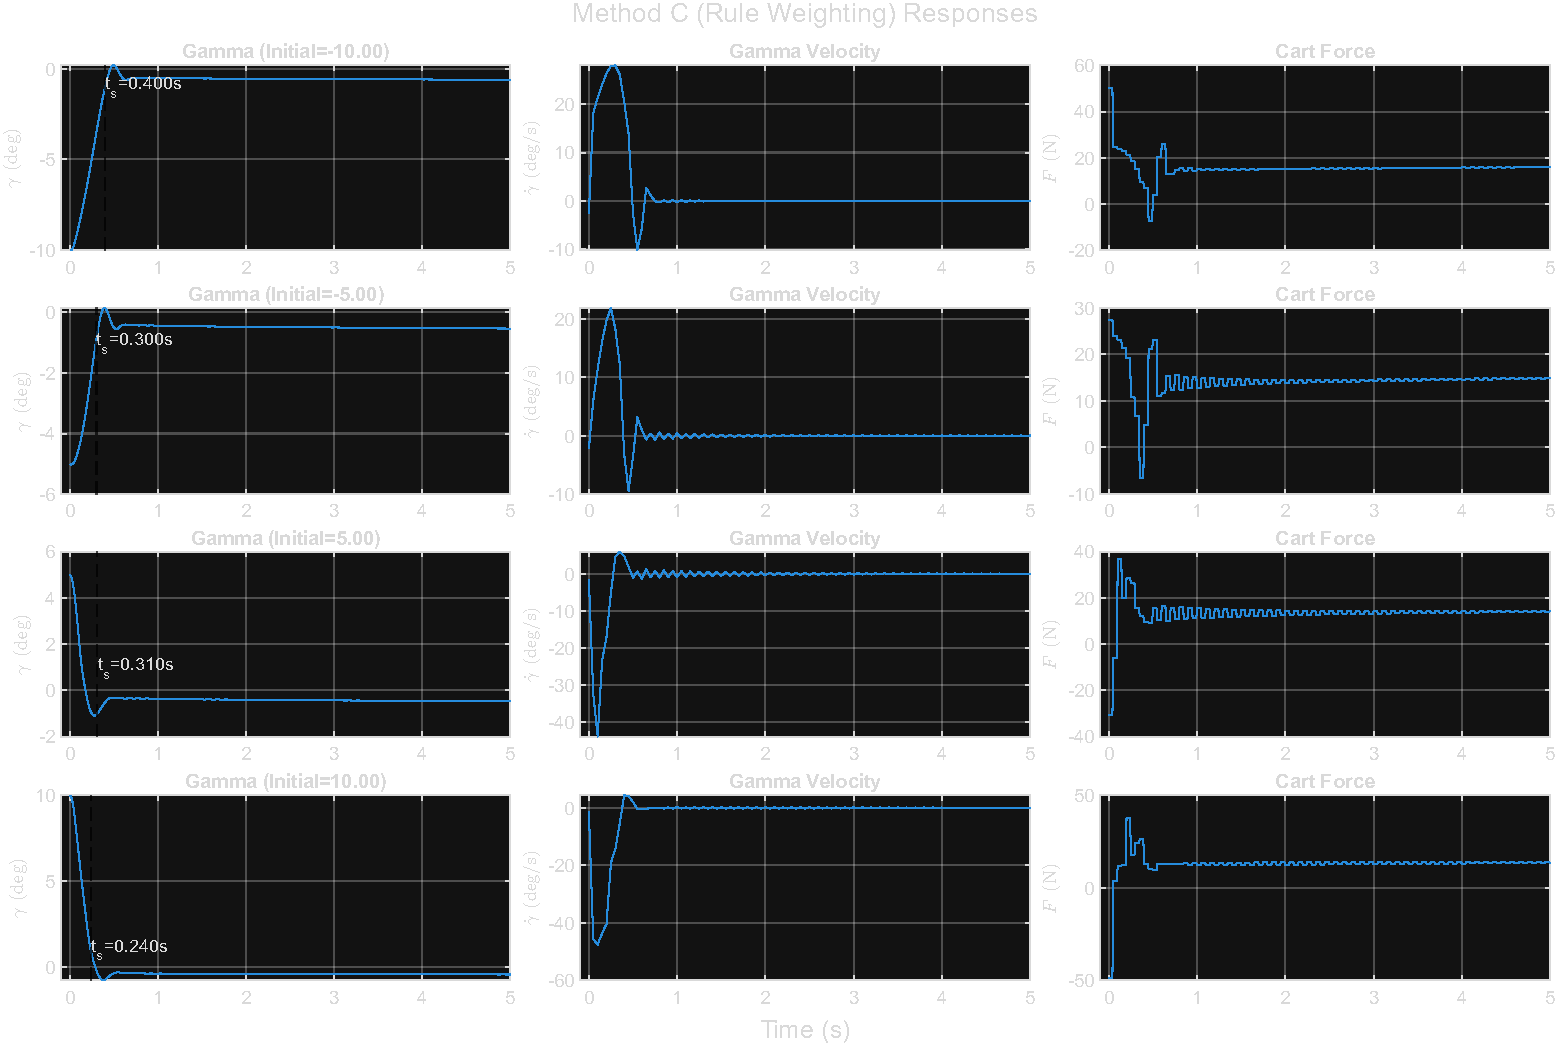
\includegraphics[width=\textwidth]{p1_responses_methodC.pdf}
\caption{Method C (final, S3) responses for the four initial angles. Compare
to the baseline in Figure~\ref{fig:baseline}: $\gam$ settles in well under
\SI{0.5}{\s} for every initial angle instead of drifting to a fixed offset,
and $\gamdot$/$f$ show no sustained chatter (contrast with S2, discussed in
the text and in Section~\ref{sec:negative}).}
\label{fig:methodc}
\end{figure}

\subsection{Method D: \todo{second method of member 1}}
\label{sec:method-d}

\paragraph{Motivation and hypothesis.} \todo{}
\paragraph{Design.} \todo{}
\paragraph{Results and interpretation.} \todo{}

\subsection{Negative results}
\label{sec:negative}

\begin{table}[H]
\centering
\small
\begin{tabular}{@{}p{2.4cm}p{4.6cm}p{8.0cm}@{}}
\toprule
\textbf{Method} & \textbf{Observed effect} & \textbf{Proposed explanation / insight gained} \\
\midrule
Method C, v1 (rule weighting, tracking-only cost; S2 in Table~\ref{tab:method-c}) &
Excellent $\ts$, overshoot and $\sse$ on $\gam$ alone, but the cart force
visibly bangs between saturation limits and tail
$\operatorname{std}(\gamdot){=}3.70\degC/\text{s}$ -- clearly sustained
chattering, even though it barely moves the report's own peak-to-peak-$\gam$
Oscillation metric. &
Several rule weights were driven to their $0.02$ floor by the optimiser,
since that minimises tracking error fastest; with weights differing by more
than an order of magnitude, \texttt{wtaver} effectively swaps between two
near-binary force levels as $p,d$ cross the boundary between two rules'
support, i.e.\ the blend becomes close to bang-bang control. Insight: an
optimisation objective built only from standard settling/overshoot/SS-error
terms is not sufficient for this problem, because none of them look at
$\gamdot$ or $f$ directly; adding explicit chattering penalties on
$\Delta f$ and tail $\Delta\gamdot$ (giving S3) fixed it, at the cost of
$\sim\!0.24\degC$ extra mean $\sse$ -- a trade accepted because ``negligible
oscillations'' is an explicit worksheet requirement and the original
Oscillation metric alone would not have caught the regression. \\
\todo{} & \todo{} & \todo{} \\
\bottomrule
\end{tabular}
\caption{Tuning attempts that did not improve performance.}
\label{tab:negative}
\end{table}

\subsection{Comparison of methods}
\label{sec:comparison}

\begin{table}[H]
\centering
\small
\begin{tabular}{@{}lcccc@{}}
\toprule
\textbf{Method} & $\Delta\ts$ (\si{\s}) & $\Delta\overshoot$ (\si{\%}) & $\Delta\sse$ (\si{\degree}) & \textbf{Significance} \\
\midrule
A & \todo{} & \todo{} & \todo{} & \todo{} \\
B & \todo{} & \todo{} & \todo{} & \todo{} \\
C & $\infty \to 0.31$ & $-12.9$ & $-1.32$ &
\parbox[t]{4.2cm}{large -- only method so far under the \SI{0.5}{\s}
target; see \S\ref{sec:method-c}} \\[0.6em]
D & \todo{} & \todo{} & \todo{} & \todo{} \\
\bottomrule
\end{tabular}
\caption{Improvement contributed by each method relative to the baseline. This
table is the core evidence of the report.}
\label{tab:comparison}
\end{table}

\section{Combined Best Model}
\label{sec:best}

\subsection{Combination and retuning}
\label{sec:combination}

\todo{Apply the successful methods together, then retune, because the
individually optimal parameters interact (worksheet Section 8, items 11--13).
Report the combined and retuned parameter set here.}

\begin{table}[H]
\centering
\small
\begin{tabular}{@{}llll@{}}
\toprule
\textbf{Term} & \textbf{Proportional error} & \textbf{Derivative error} & \textbf{Force (\si{\N})} \\
\midrule
NB & \todo{} & \todo{} & \todo{} \\
NS & \todo{} & \todo{} & \todo{} \\
ZO & \todo{} & \todo{} & \todo{} \\
PS & \todo{} & \todo{} & \todo{} \\
PB & \todo{} & \todo{} & \todo{} \\
\bottomrule
\end{tabular}
\caption{Best model membership function parameters.}
\label{tab:best-params}
\end{table}

\begin{table}[H]
\centering
\small
\begin{tabular}{@{}cccccc@{}}
\toprule
$\gam_0$ (\si{\degree}) & $\ts$ (\si{\s}) & $\overshoot$ (\si{\%}) & $\sse$ (\si{\degree}) & Oscillation & Verdict \\
\midrule
$-10$ & \todo{} & \todo{} & \todo{} & \todo{} & \todo{} \\
$-5$  & \todo{} & \todo{} & \todo{} & \todo{} & \todo{} \\
$5$   & \todo{} & \todo{} & \todo{} & \todo{} & \todo{} \\
$10$  & \todo{} & \todo{} & \todo{} & \todo{} & \todo{} \\
\bottomrule
\end{tabular}
\caption{Best model performance. Target: $\ts < \SI{0.5}{\s}$, no overshoot,
zero steady-state error for all four initial angles.}
\label{tab:best}
\end{table}

\begin{figure}[H]
\centering
\todo{Insert the best-model response figure here (plot the four responses and
mark $\ts$).}
\caption{Best model responses.}
\label{fig:best}
\end{figure}

\subsection{Explaining the interactions}
\label{sec:interactions}

\todo{Explain, with theory and evidence, why the combined optimum differs from
the per-method optima: which universes trade off against each other, and which
metric each trade-off is governed by.}

\subsection{Sensitivity and robustness}
\label{sec:robustness}

\todo{Perturb the chosen parameters slightly and repeat the simulation to show
the result is not a knife-edge optimum. Optionally re-run with sensor noise and
with a mismatched slope angle.}\\
\todo{Candidate robustness checks: $\pm\SI{5}{\%}$ perturbation of the slope
angle $\phi$; the noise lines already present in the worksheet; a cart-mass
mismatch.}

\section{Conclusion}
\label{sec:conclusion}

\todo{State the best model found, its four metrics, the mechanism that
explains the improvement, and the limitations of the study (fixed plant
parameters, single seed, saturation, model-based simulation).}

% =============================================================================
% BACK MATTER
% =============================================================================
\clearpage
\section*{Declarations}
\addcontentsline{toc}{section}{Declarations}
\begin{itemize}[leftmargin=*]
  \item All simulations reported here were produced by the submitted
        \texttt{p1\_team16.mlx} worksheet with the seed
        $\mathrm{rng}(\mathrm{sum}([286716, 284748]))$.
  \item \todo{AI-tool / collaboration declaration as required by the course.}
  \item \todo{Statement on data availability, e.g.\ sweep data in
        Appendix~\ref{app:data}.}
\end{itemize}

\clearpage
\addcontentsline{toc}{section}{References}
\bibliographystyle{plain}
\bibliography{references}

\clearpage
\appendix
\section{Full Tuning Data}
\label{app:data}

\todo{Complete sweep tables for every experiment, including the runs that are
not discussed in the main body (worksheet Section 8, item 5).}

\section{Membership Function Figures}
\label{app:figs}

\todo{MF plots and control surfaces for each method and for the best model,
one page each.}

\section{Worksheet Code Listing}
\label{app:code}

\todo{Paste the submitted worksheet listing
(\texttt{initFis}, \texttt{controller}, seeding and simulation harness).}

\end{document}
